\documentclass{beamer}

\usepackage{beamerthemesplit}
\usetheme{Singapore} %Copenhagen}
%\usecolortheme{whale}

%\usepackage[T2A]{fontenc}
%\usepackage[utf8]{inputenc}
%\usepackage[russian]{babel}

\usepackage[main=russian,english]{babel}   %% загружает пакет многоязыковой вёрстки
\usepackage{fontspec}      %% подготавливает загрузку шрифтов Open Type, True Type и др.
\defaultfontfeatures{Ligatures={TeX},Renderer=Basic}  %% свойства шрифтов по умолчанию
\setmainfont{Times New Roman} %% задаёт основной шрифт документа
%\usefonttheme{professionalfonts}% SOLUTION
\usefonttheme{serif}

\usepackage{hyperref}
\usepackage{textcomp}
\usepackage{amssymb,amsmath}
%\usepackage{animate}
%\usepackage{longtable}
\usepackage{xcolor}

%\usepackage{pgffor}
\usepackage{enumitem}


\newcounter{N}

%% Форматирование окружения itemize
%\usepackage{ragged2e}
%\let\olditem\item
%\renewcommand\item{\olditem\justifying}

\usepackage{ mathrsfs }
\newcommand{\Rho}{\mathscr{P}}

\newcommand{\argxi}{(\xi^1,\xi^2,\xi^3)}
\newcommand{\argx}{(x^1,x^2,x^3)}

\newcommand{\argxiv}{(\vec{\xi})}
\newcommand{\argxv}{(\vec{x})}


\newcommand{\argxbarn}{(\bar{x}^1,\bar{x}^2,\ldots, \bar{x}^n)}
\newcommand{\argxn}{(x^1, x^2,\ldots, x^n)}

\newcommand{\argtxi}{(t, \xi^1,\xi^2,\xi^3)}
\newcommand{\argtoxi}{(t_0, \xi^1,\xi^2,\xi^3)}

\newcommand{\argtxiv}{(t, \vec{\xi})}
\newcommand{\argtoxiv}{(t_0, \vec{\xi})}


\newcommand{\argtx}{(t, x^1,x^2,x^3)}
\newcommand{\argtox}{(t_0, x^1,x^2,x^3)}

\newcommand{\argtxv}{(t, \vec{x})}
\newcommand{\argtoxv}{(t_0, \vec{x})}


\newcommand{\pd}[2]{\frac{\partial #1}{\partial #2}}
\newcommand{\pdk}[2]{\frac{\partial^2 #1}{\partial #2^2}}

\newcommand{\grad}{\operatorname{grad}}
\newcommand{\rot}{\operatorname{rot}}
\newcommand{\divo}{\operatorname{div}}

\title[]{Вихревые течения идеальной жидкости}

\author[]{ {\em Верещагин Антон Сергеевич}
\\
канд. физ.-мат. наук, старший преподаватель\\
\bigskip
Кафедра аэрофизики и газовой динамики ФФ НГУ}

\usebackgroundtemplate{\includegraphics[width=\paperwidth]{../img/background.png}}

\begin{document}
	
\frame{\titlepage}


\frame{
	\frametitle{Аннотация}
	\parbox{\textwidth}{
	Вихревые течения. Вихревые линия, трубка. Теорема о циркуляции вектора вихря. Теорема о проихводной циркуляции скорости. Теорема Томсона. Теорема Лагранжа. Первая и вторая теоремы Гельмгольца. 
	}
}


\frame{
	\frametitle{ Потенциальные и вихревые течения идеальной жидкости}
	
	\begin{exampleblock}{Определение}
		\parbox{\textwidth}{
			
			Течение идеальной жидкости называется \alert{вихревым}, если вектор $\vec{\Omega} = \rot \vec{v}$ в некоторых точках исследуемой области отличен от нулевого.
					
			\pause	
			Выражение для компонент вектора вихря
			\[
			\Omega_x = \pd{v_z}{y}-\pd{v_y}{z},\quad
			\Omega_y = \pd{v_x}{z}-\pd{v_z}{x},\quad
			\Omega_z = \pd{v_y}{x} -\pd{v_x}{y}.
			\]		
			
			\pause	
			Если же в исследуемой области везде $\vec{\Omega}=0$, тогда течение в этой области называется потенциальным, и существует потенциал $\varphi$ такой, что
			\[
			\vec{v} = \nabla\varphi.
			\]
			Справедливо и обратное утверждение.
			

			
		}
	\end{exampleblock}
	
}

\frame{
	\frametitle{ Пример вихревого течения }
	
	
	\begin{columns}
		\begin{column}{0.5\textwidth}
			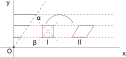
\includegraphics[width=\textwidth]{../img/rot_example.pdf}	
		\end{column}
		\begin{column}{0.5\textwidth}
		Движение жидкости слоями
		\[
		v_x = ay,\quad
		v_y=0,\quad
		v_z=0.
		\]	
		Вихрь скорости 
		\[
			\Omega_x = 0,\quad
			\Omega_y = 0,\quad
			\Omega_z = -a.
		\]
		\end{column}
	\end{columns}

	\begin{exampleblock}{Описание}
		\parbox{\textwidth}{
			По теореме Кельвина-Гельмгольца о скорости деформируемой частицы квадрат $I$  переходит в параллелограмм $II$ посредством сдвига вдоль оси $x$, поворота как твердого тела по указанной стрелке и чистой деформации в виде сжатия вдоль линии $\alpha$ и растяжения вдоль линии $\beta$.
			
		}
	\end{exampleblock}

}

\frame{
	\frametitle{Вихревые линии и вихревые трубки}
	
	\begin{exampleblock}{Определение}
		\parbox{\textwidth}{
			\alert{Вихревой линиией} называется такая линия, во всякой точке которой вихрь скорости $\vec{\Omega}$ направлен по касательной к этой линии. 			
		}
	\end{exampleblock}

	\begin{exampleblock}{Уравнения вихревой линии}
		\parbox{\textwidth}{
			\[
			\frac{dx}{\Omega_x}=\frac{dy}{\Omega_y} = \frac{dz}{\Omega_z}.
			\]
		}
	\end{exampleblock}


}

\frame{
	\frametitle{ Вихревая трубка }
	
	\begin{exampleblock}{Определение}
		\parbox{\textwidth}{
			\alert{Вихревой трубкой} называется совокупность точек пространства, ограниченных вихревыми линиями, проведёнными через заданный замкнуты контур.
		}
	\end{exampleblock}
	
	\bigskip
	\centering
	\includegraphics[width=0.7\textwidth]{../img/rot_tube.pdf}
	

}

\frame{
	\frametitle{ Циркуляция скорости и теорема Стокса}
	
	\begin{exampleblock}{Определение}
		\parbox{\textwidth}{
			\alert{Циркуляцией скорости} $\Gamma$ по замкнутому контуру называется линейный интеграл
			\[
			\Gamma = \oint\limits_C \vec{v}\cdot d\vec{l} = \oint\limits_C v_x dx + v_y dy + v_z dz.
			\]
		}
	\end{exampleblock}
	\begin{exampleblock}{Теорема Стокса}
		\parbox{\textwidth}{
			Циркуляция вектора по замкнутому контуру равна потоку ротора этого вектора через площадку, ограниченную этим контуром:
			\[
			\oint\limits_C \vec{v}\cdot d\vec{l} = 
			\int\limits_S (\vec{n} \cdot \rot \vec{v}) dS,
			\]
			где вектор $\vec{n}$ -- вектор единичной нормали к $S$, направленный по правилу буравчика. 
			
		}
	\end{exampleblock}
}

\frame{
	\frametitle{ Интенсивность вихревой трубки }
	
	\begin{exampleblock}{Определение}
		\parbox{\textwidth}{
			Интенсивностью вихревой трубки называется поток вектора вихря $\Omega$ через сечение вихревой трубки 
			\[
			I=\int\limits_S \vec{\Omega} \cdot \vec{n} dS.
			\]
			
		}
	\end{exampleblock}


}

\frame{
	\frametitle{ Теорема о постоянстве циркуляции для вихревой трубки}
	
	\begin{exampleblock}{Теорема}
		\parbox{\textwidth}{
			Циркуляция вектора скорости по любому замкнутому контуру, охватывающему данную вихревую трубку постоянна.
		}
	
	\bigskip\pause
	\end{exampleblock}
		\begin{columns}
		\begin{column}{0.5\textwidth}
			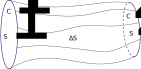
\includegraphics[width=\textwidth]{../img/circul_tube.pdf}
		\end{column}
		\begin{column}{0.5\textwidth}
		\parbox{\textwidth}{
		Рассмотрим вихревую трубку $V$,	ограниченную с торцов сечениями $S_1$, $S_2$ и боковой поверхностью $\Delta S$. Сечения $S_1$, $S_2$ пересекаются с $\Delta S$ по контурам $C_1$ и $C_2$.
		}
		
		\end{column}
	\end{columns}

	\pause
	\bigskip
	\[
	0 = \int\limits_V \divo \rot \vec{v} \, dV= 
	\int\limits_V \divo \vec{\Omega} dV=
	\int\limits_S \vec{\Omega}\cdot \vec{n} dS
	\]
}

\frame{
	\frametitle{ Теорема о постоянстве циркуляции для вихревой трубки: доказательство }
	\centering		
	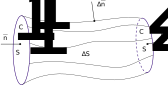
\includegraphics[width=0.5\textwidth]{../img/circul_tube_normals.pdf}
	
	\bigskip
	\parbox{\textwidth}{
	\[
	\int\limits_S \vec{\Omega}\cdot \vec{n} dS = 
	\int\limits_{S_1} \vec{\Omega}\cdot \vec{n}_1 dS+
	\int\limits_{S_2} \vec{\Omega}\cdot \vec{n}_2 dS+
	\int\limits_{\Delta S} \vec{\Omega}\cdot \Delta\vec{n} dS.
	\]	
	Т.к. на боковой поверхности вихревой трубки $\Delta S$ вектора $\vec{\Omega}$ и $\Delta\vec{n}$ ортогональны, то последний интеграл равен 0.
	}
	
	
}


\frame{
	\frametitle{ Теорема о постоянстве циркуляции для вихревой трубки: доказательство }
	\centering		
	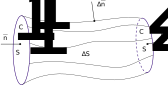
\includegraphics[width=0.5\textwidth]{../img/circul_tube_normals.pdf}
	
	\bigskip
	\parbox{\textwidth}{
		Таким образом, используя теорему Стокса, имеем
		\[
		0 = 
		\int\limits_{S_1} \vec{\Omega}\cdot \vec{n}_1 dS+
		\int\limits_{S_2} \vec{\Omega}\cdot \vec{n}_2 dS=
		\oint\limits_{C_1} \vec{v} \cdot d\vec{l} -
		\oint\limits_{C_2} \vec{v} \cdot d\vec{l}. 	
		\]
		В последнем равенстве появился знак минус, потому что нормали $\vec{n}_1$ и $\vec{n}_2$ направлены в разные стороны. Так как контуры $C_1$ и $C_2$ выбраны произвольно, то справедливо утверждение теоремы. 
	}
	
	
}



\frame{
	\frametitle{ Теорема о постоянстве циркуляции для вихревой трубки: доказательство }
	\centering		
	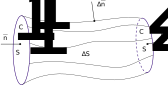
\includegraphics[width=0.5\textwidth]{../img/circul_tube_normals.pdf}
	
	\bigskip
	\parbox{\textwidth}{
		Таким образом, используя теорему Стокса, имеем
		\[
		0 = 
		\int\limits_{S_1} \vec{\Omega}\cdot \vec{n}_1 dS+
		\int\limits_{S_2} \vec{\Omega}\cdot \vec{n}_2 dS=
		\oint\limits_{C_1} \vec{v} \cdot d\vec{l} -
		\oint\limits_{C_2} \vec{v} \cdot d\vec{l}. 	
		\]
		
		Дополнительно показано, что интенсивность вихревой трубки одна и та же в любом сечении. 
	}
	
	
}

\frame{
	\frametitle{ Теорема о производной циркуляции скорости }
	
	\begin{exampleblock}{Теорема}
		\parbox{\textwidth}{
			Производная по времени от циркуляции скорости $\vec{v}$ по некоторому замкнутому контуру равна циркуляции от ускорения $d\vec{v}/dt$ по тому же контуру
			
			\[
			\frac{d}{dt}\oint\limits_L\vec{v}\cdot d\vec{s} =
			\oint\limits_L\frac{d\vec{v}}{dt}\cdot d\vec{s}.
			\]
		}
	\end{exampleblock}
	
}

\frame{
	\frametitle{ Теорема о производной циркуляции скорости: доказательство }
	
	\begin{columns}
		\begin{column}{0.5\textwidth}
			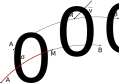
\includegraphics[width=\textwidth]{../img/J_def.pdf}
		\end{column}
		\begin{column}{0.5\textwidth}
			\parbox{\textwidth}{
				Рассмотрим в момент времени $t_0$ какую-нибудь линию $A_0B_0$, проведённую в жидкости, состоящую из жидких частиц, которая в момент времени $t$ перейдёт в другую линию $AB$. Рассмотрим линейный интеграл от скорости по этой кривой

			}
		
	
		\end{column}
	\end{columns}

	\medskip
	\[
	J = \int\limits_{AB}\vec{v}\cdot d\vec{s}
	\]

	
}

\frame{
	\frametitle{ Теорема о производной циркуляции скорости: доказательство }
	\parbox{\textwidth}{
		В момент времени $t'=t+\Delta t$ линия $AB$ перейдёт в $A'B'$ и можно определить $J'$
		\[
		J' =  \int\limits_{A'B'}\vec{v}'\cdot d\vec{s}
		\]
		
		\pause
		Определим производную по времени от линейного интеграла	$\displaystyle\frac{dJ}{dt}$ как 
		\[
		\frac{dJ}{dt} = \lim\limits_{\Delta\to 0}\frac{J'-J}{\Delta t}.
		\]
	}
}

\frame{
	\frametitle{ Теорема о производной циркуляции скорости: доказательство }
	
	\begin{columns}
		\begin{column}{0.5\textwidth}
			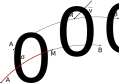
\includegraphics[width=\textwidth]{../img/J_def.pdf}
		\end{column}
		\begin{column}{0.5\textwidth}
			\parbox{\textwidth}{
				Параметризуем отрезок $A_0B_0$ параметром $\sigma$ равным расстоянию от выбранной точки $M_0$ вдоль дуги $A_0M_0$. Тогда точку $M$ отрезка $AB$ в момент времени $t$ можно однозначно определить с помощью следующих соотношений:
			}
			
			
		\end{column}
	\end{columns}
	
	\[
		x = x(\sigma, t),\quad
		y = y(\sigma, t),\quad	
		z = z(\sigma, t)
	\]
	или
	\[
	\vec{r} = \vec{r}(\sigma,t)\quad
	(0\leq \sigma \leq \sigma_0, \, t \geq t_0),
	\]
	при этом
	\[
		\vec{r}(0, t) = A,\quad
		\vec{r}(\sigma,t) = M,\quad
		\vec{r}(\sigma_0,t)=B.
	\]
	
	
}

\frame{
	\frametitle{  Теорема о производной циркуляции скорости: доказательство }
	
	\parbox{\textwidth}{
	Скорости жидких частиц отрезка $AB$ также можно параметризовать через $\sigma$ и $t$:
	\[
		\vec{v} = \vec{v}(\sigma,t).
	\]
		
	\pause
	Линейный интеграл $J$, используя $\sigma$ и $t$ можно переписать форме
	\[
	J = \int\limits_{0}^{\sigma_0}
	\left(v_x\pd{x}{\sigma} + v_y\pd{y}{\sigma} + v_z\pd{z}{\sigma}\right)d\sigma=
	\int\limits_{0}^{\sigma_0} \left( \vec{v} \cdot \pd{\vec{r}}{\sigma} \right) d\sigma,
	\]
	где предел интегрирования не зависит от переменной $t$.
	}
	
}

\frame{
	\frametitle{ Теорема о производной циркуляции скорости: доказательство }
	\parbox{\textwidth}{
	Рассмотрим производную от $J$ по $t$:
	\[
	\frac{dJ}{dt} = 
	\int\limits_{0}^{\sigma_0} \left(\pd{\vec{v}}{t}\cdot\pd{\vec{r}}{\sigma}\right) d\sigma +
	\int\limits_{0}^{\sigma_0} \left( \vec{v}\cdot \frac{\partial^2\vec{r} }{\partial\sigma \partial t} \right) d\sigma =
	\]
	\[
	=
	\int\limits_{0}^{\sigma_0} \left(\vec{a}\cdot\pd{\vec{r}}{\sigma}\right) d\sigma +
	\int\limits_{0}^{\sigma_0} \left( \vec{v}\cdot \pd{\vec{v}}{\sigma} \right) d\sigma.
	\]
	Здесь
	\[
		\pd{}{t}\vec{r}(\sigma,t) = \vec{v}(\sigma,t),\quad
		\frac{\partial^2 }{\partial\sigma \partial t}\vec{r} (\sigma,t) =  \pd{}{\sigma}  \vec{v}(\sigma,t),\quad
		\pd{ }{t} \vec{v}(\sigma,t) = \vec{a}(\sigma,t),
	\]
	где $\vec{a}$ -- ускорение жидкой частицы.
	}
	
}


\frame{
	\frametitle{Теорема о производной циркуляции скорости: доказательство }
	
	\parbox{\textwidth}{
	Рассмотрим отдельно каждое слагаемое.
	\[
	\int\limits_{0}^{\sigma_0} \left(\vec{a}\cdot\pd{\vec{r}}{\sigma}\right) d\sigma=
	\int\limits_{AB}\vec{a} \cdot d\vec{s} =
	\int\limits_{AB}\frac{d\vec{v}}{dt} \cdot d\vec{s},
	\]
	в последнем равенстве $d/dt$ -- полная производная.
	
	\pause
	\[
	\int\limits_{0}^{\sigma_0} \left( \vec{v}\cdot \pd{\vec{v}}{\sigma} \right) d\sigma=
	\frac{1}{2}\int\limits_{0}^{\sigma_0} \pd{}{\sigma}
	\left( 
	\vec{v}\cdot\vec{v}
	\right) d\sigma =
	\frac{v_B^2}{2} - \frac{v_A^2}{2},
	\]
	где $\vec{v}_B=\vec{v}(\sigma_0,t)$, $\vec{v}_A=\vec{v}(0,t)$ -- скорости жидких частиц в точках $B$, $A$.
	}
	
	
}


\frame{
	\frametitle{Теорема о производной циркуляции скорости: итог }
	
	\parbox{\textwidth}{
		Подводя итог вышесказанного
		\[
		\frac{dJ}{dt} =
		\int\limits_{AB}\frac{d\vec{v}}{dt} \cdot d\vec{s} +
		\frac{v_B^2}{2} - \frac{v_A^2}{2}.
		\]
		

		
	}
		\pause
	\begin{exampleblock}{Результат}
		\parbox{\textwidth}{
			
		Если в качестве линии $AB$ рассматривать замкнутый контур $L$, тогда точки $A$ и $B$ совпадают и 
		\[
		\frac{d}{dt}\oint\limits_L \vec{v} \cdot d\vec{s} =
		\oint\limits_L \frac{d\vec{v}}{dt} \cdot d\vec{s}.
		\]	
		}
	\end{exampleblock}
}

\frame{
	\frametitle{ Теорема Томсона }
	
	\begin{exampleblock}{Теорема}
		\parbox{\textwidth}{
			Если массовые силы допускают потенциал, а идеальная жидкость баротропна, то циркуляция скорости по любому замкнутому контуру во все время движения жидкости остаётся неизменной. 
		}
	\end{exampleblock}
	
}

\frame{
	\frametitle{ Теорема Томсона: доказательство }
	
	\begin{exampleblock}{Уравнение движения}
		\parbox{\textwidth}{
			Для баротропного течения идеальной жидкости с потенциальными массовыми силами уравнение движения допускает следующее упрощение (см. предыдущую лекцию)
			\[
			\frac{d\vec{v}}{dt} = -\grad\left( \Rho(p) + \Pi \right).
			\]
			Здесь 
			\[
			\Rho(p) = \int\limits_{p_0}^{p} \frac{dp}{\rho},\quad
			\vec{f} = -\nabla \Pi,
			\]
			где $\Rho(p)$ -- функция давления; $\vec{f}$, $\Pi$ -- вектор и потенциал объёмных сил.
			
		}
	\end{exampleblock}
}

\frame{
	\frametitle{ Теорема Томсона: доказательство }

	\parbox{\textwidth}{
	Рассмотрим производную циркуляции вектора скорости по замкнутому контуру $L$. По теореме о циркуляции и закона движения имеем
	\[	\frac{d}{dt}\oint\limits_L \vec{v} \cdot d\vec{s} =
	\oint\limits_L \frac{d\vec{v}}{dt} \cdot d\vec{s} = 
%	\]
%	\[
%	=
	-\oint\limits_L \grad\left( \Rho(p) + \Pi \right) \cdot d \vec{s} = 
%	-\oint\limits_L d \left( \Rho(p) + \Pi \right) = 
	0.
	\]
	}

	\pause
	\begin{exampleblock}{Результат}
		\parbox{\textwidth}{
		Таким образом,
		\[
			\oint\limits_L \vec{v} \cdot d\vec{s} = const.
		\]
		}
	\end{exampleblock}


	
}

\frame{
	\frametitle{ Теорема Лагранжа }
	
	\begin{exampleblock}{Теорема}
		\parbox{\textwidth}{
			Если при баротропном течении идеальной жидкости в потенциальном внешнем поле в начальный момент времени какие-то жидкие частицы не имели завихрённости, то её в них не было раньше и не будет позже.
		}
	\end{exampleblock}\pause

	\begin{exampleblock}{Теорема (альтернативная формулировка)}
	\parbox{\textwidth}{
		Если баротропное течении идеальной жидкости в потенциальном внешнем поле в начальный момент времени было потенциально в какой-то момент времени, то оно останется потенциальным в любой другой и далее.
	}
\end{exampleblock}
}

\frame{
	\frametitle{Теорема Лагранжа: доказательство }
	
	\parbox{\textwidth}{
		Пусть в некоторый момент времени в каком-то объёме жидкости $\vec{\Omega}=0$, тогда по теореме Стокса циркуляция по любому замкнутому контуру в этой области равна $0$. По теореме Томсона циркуляция для такой жидкости не меняется от времени, а значит, для рассматриваемых жидких частиц циркуляция в любой другой момент времени тоже равна 0. 
		
		\medskip\pause
		В окрестности выбранной жидкой частицы рассмотрим всевозможные маленькие площадки $S$ с нормалью $\vec{n}$ и контуром $L$, тогда по теореме Стокса
		\[
		\int\limits_{S} \vec{\Omega}\cdot \vec{n} dS = \oint\limits_{L} \vec{v}\cdot d\vec{s} = 0,
		\]
		а следовательно и
		\[
		\vec{\Omega} = 0.
		\]
	}
	
}

\frame{
	\frametitle{ Первая теорема Гельмгольца}
	
	\begin{exampleblock}{Теорема (о сохранении вихревых линий)}
		\parbox{\textwidth}{
			В баротропном течении идеальной жидкости в потенциальном внешнем поле частицы жидкости, образующие в некоторый момент вихревую линию, во всё время движения будут образовывать вихревую линию.			
		}
	\end{exampleblock}
	
}

\frame{
	\frametitle{ Первая теорема Гельмгольца: доказательство }
	
	\parbox{\textwidth}{
	Рассмотрим \alert{вихревую поверхность} -- поверхность, образованная вихревыми линиями, проведёнными через некоторую линию в пространстве, которая сама не является вихревой линией.
	В каждой точке поверхности вектор $\vec{\Omega}$ будет ортогонален вектору нормали $\vec{n}$ к этой поверхности. Покажем, что частицы, составляющие вихревую поверхность в какой-то момент времени будет ей является и далее. \pause
	
	\medskip
	Рассмотрим на поверхности контур $L$, образующий на поверхности площадку $S$, и посчитаем циркуляцию вектора скорости по этому контуру
	\[
	\oint\limits_{L}\vec{v}\cdot d\vec{s} = \int\limits_S \vec{\Omega}\cdot \vec{n} dS = 0.
	\]
	Последнее равенство выполнено в силу того, что $\vec{\Omega} \perp \vec{n}$.
		
	}
	
}

\frame{
	\frametitle{ Первая теорема Гельмгольца: доказательство }
	\parbox{\textwidth}{
		В последующие моменты времени поверхность перейдёт в другую поверхность, а контур $L$ в контур $L'$, ограничивающий площадку $S'$. По теореме Томсона циркуляция по контуру $L'$ равна циркуляции по контуру $L$ и равна 0, следовательно, используя теорему Стокса
		\[
		0 = \oint\limits_{L'} \vec{v'}\cdot d\vec{s} = 
		\int\limits_{S'} \vec{\Omega'}\cdot \vec{n}' dS,
		\]
		где $\vec{v}'$, $\vec{\Omega}'$ -- вектора скорости и вихря в последующий рассматриваемый момент времени; $\vec{n}'$ -- нормаль к поверхности, образованной теми же самыми жидкими частицами.
		\pause
		
		\medskip
		Т.к. в последнем равенстве $S'$ можно взять сколь угодно маленькую, то $\vec{\Omega}'\perp \vec{n}'$. Таким образом, поверхность, образованная теми же самыми жидкими частицами, тоже будет вихревой поверхностью.
	}
	
}

\frame{
	\frametitle{ Первая теорема Гельмгольца: доказательство }
	\parbox{\textwidth}{
	Рассмотрим вихревую линию $l$, являющуюся пересечением двух вихревых поверхностей $S$ и $\Sigma$ в какой-то момент времени. В следующий рассматриваемый момент времени она перейдёт в линию $l'$, являющуюся пересечением вихревых поверхностей $S'$ и $\Sigma'$, в которые перейдут вихревые поверхности $S$ и $\Sigma$. \pause
	
	\medskip
	В каждой точке кривой $l'$ вихрь $\vec{\Omega}'$ лежит в касательной плоскости $S'$ и $\Sigma'$, а значит и является касательным вектором для кривой $l'$.
	
		
	}\pause

	\medskip
	\begin{exampleblock}{Результат}
		\parbox{\textwidth}{
			В рассматриваемом случае каждая вихревая линия перемещается в пространстве вместе с жидкими частицами, её образующими. Это свойство называется \alert{сохраняемостью вихревых линий}.
		}
	\end{exampleblock}
	
}

\frame{
	\frametitle{ Первая теорема Гельмгольца: следствие }
	
	\begin{exampleblock}{Теорема}
		\parbox{\textwidth}{
		В баротропном течении идеальной жидкости в потенциальном внешнем поле частицы жидкости, образующие в некоторый момент вихревую трубку, во всё время движения будут образовывать вихревую трубку.	
		}
	\end{exampleblock}
}

\frame{
	\frametitle{ Вторая теорема Гельмгольца }
	
	\begin{exampleblock}{Теорема}
		\parbox{\textwidth}{
		В баротропном течении идеальной жидкости в потенциальном внешнем поле интенсивность выделенной вихревой трубки будет сохраняться во время её движения.			
		}
	\end{exampleblock}
	
	\pause
	\begin{exampleblock}{Доказательство}
		\parbox{\textwidth}{
			Интенсивность вихревой трубки определяется циркуляцией по любому замкнутому контуру этой трубки
			\[
			\Gamma = \oint\limits_L \vec{v}\cdot d\vec{s},
			\]
			которая по теореме о сохранении циркуляции будет равна циркуляции по контуру трубки тока, образованной из тех же жидких частиц в последующие моменты времени. Т.е. интенсивность её будет такой же.
		}
	\end{exampleblock}

	
}



\frame{
	\frametitle{ Литература }
	\begin{itemize}[partopsep=1pt,label=\textbullet]
		\item {\em Кочин~Н.~Е., Кибель~И.~А., Розе~Н.~В.} Теоретическая гидромеханика. М.:Гос. издат. физ.-мат. лит., 1963.
	\end{itemize}
}
\end{document}
